\documentclass[a4j,dvipdfmx]{jsreport}
\usepackage{listings,jlisting,color}
\lstset{
  aboveskip=20pt,
  belowskip=20pt,
}
\lstdefinestyle{source}{%
  language=Java,
  basicstyle=\ttfamily\small,
  numbers=left,
  numberstyle=\ttfamily,
  xleftmargin=2em,
  basewidth=.51em,
  frame=shadowbox,
  rulesepcolor=\color{black},
}
\lstdefinestyle{result}{%
  basicstyle=\ttfamily\small,
  xleftmargin=2em,
  basewidth=.51em,
  frame=single,
  frameround=tttt,
}
%\renewcommand{\lstlistingname}{\textbf{Source Code.}}
\makeatletter
    \AtBeginDocument{
    \renewcommand*{\thelstlisting}{\arabic{lstlisting}}}
\makeatother

\usepackage{float}
\usepackage{tabularx}
\usepackage{subfigure}
\usepackage{tasks}
\usepackage{graphicx}
\usepackage{amsmath}
\usepackage{url}
%\usepackage[dvipdfmx]{hyperref}

\title{
データ構造とアルゴリズム レポート課題
\large{\\---ソーティングアルゴリズムに関する検証と考察---}
}
\author{34719034 水野翔真}
\date{\today}
\begin{document}
\maketitle
\tableofcontents

\chapter{はじめに}
\section{レポート概要}
本レポートは、2023年度 前期 データ構造とアルゴリズムにて出された課題について纏めたレポートである。本レポートは、はじめに, 実験, 追加実験, まとめの4部構成である。
\section{実行環境}
円滑なデータの習得とレポート作成のために、本課題はCSE上ではなく著者の所有するローカルマシンで遂行された。
本課題は特に明記のない限り以下の環境で実行されることを予め断っておく。\\
MacBook Pro 14(2021モデル)\\
SoC:M1pro(CPU 8コア8スレッド(P core:3.2Ghz, E core:2.06Ghz), RAM:LPDDR5-6400 16GB)\\java11.0.17

\chapter{実験}
\section{実験概要}
以下では課題の内容について説明する。
\subsection{実装対象}
著者は学籍番号が $34719034 \equiv 2 \, (mod4)$ であるので、バブルソート, クイックソート, 基数ソートについてプログラムの実装した。
\subsection{実験対象}
CSE上の、\textasciitilde ebn02865/lecture/data-algo/ にあるdata\_80MB.zip を展開した中にある以下の50個のデータについて実験対象のデータとする\\

\settasks{counter-format=$\bullet$}
\settasks{label-width=6pt}
\begin{tasks}(5)
\task 10000\_0
\task 10000\_1
\task 10000\_2
\task 10000\_3
\task 10000\_4
\task 10000\_0\_almost
\task 10000\_1\_almost
\task 10000\_2\_almost
\task 10000\_3\_almost
\task 10000\_4\_almost
\task 50000\_0
\task 50000\_1
\task 50000\_2
\task 50000\_3
\task 50000\_4
\task 50000\_0\_almost
\task 50000\_1\_almost
\task 50000\_2\_almost
\task 50000\_3\_almost
\task 50000\_4\_almost
\task 100000\_0
\task 100000\_1
\task 100000\_2
\task 100000\_3
\task 100000\_4
\task 100000\_0\_almost
\task 100000\_1\_almost
\task 100000\_2\_almost
\task 100000\_3\_almost
\task 100000\_4\_almost
\task 500000\_0
\task 500000\_1
\task 500000\_2
\task 500000\_3
\task 500000\_4
\task 500000\_0\_almost
\task 500000\_1\_almost
\task 500000\_2\_almost
\task 500000\_3\_almost
\task 500000\_4\_almost
\task 1000000\_0
\task 1000000\_1
\task 1000000\_2
\task 1000000\_3
\task 1000000\_4
\task 1000000\_0\_almost
\task 1000000\_1\_almost
\task 1000000\_2\_almost
\task 1000000\_3\_almost
\task 1000000\_4\_almost
\end{tasks}

\newpage
\subsection{実験方法}
以下では簡単な実験方法について示す。
\begin{enumerate}
\item data\_80MB.zip をCSEからコピーし、展開後 data-algoディレクトリを任意の階層に配置する
\item ソートアルゴリズムの実装とソートを実行するためのテスターを実装する
\item コンパイルしたソートプログラムとソート対象のデータを分かりやすいように、data-algoディレクトリ内にprogramというディレクトリを作成しそこに配置する
\item ターミナルにてテスターを実行し、ソートにかかる時間を計測する
\item テスターが終了したら、得られた計測データをもとに考察をする
\end{enumerate}

\subsection{実装プログラム}
以下に今回の実装したプログラムについて示す。\par
プログラムが長いため一部移して示す。
\subsubsection{テスターのソースコード}
\lstset{caption=テスター,firstnumber=1}
\begin{lstlisting}[style=source]
import java.io.*;

class data_algo_tester extends Thread {
        public static void main(String arg[]) {
                int sortTarget;
                String SortTarget = "";
                int csvCount = 0;
                for (sortTarget = 0; sortTarget < 3; sortTarget++) {
                        int dataAmount = 0;
                        for (int dataAmountNum = 0; dataAmountNum < 5; dataAmountNum++) {
                                // 読み取るデータの数を変えます
                                switch (dataAmount) {
                                        case 0:
                                                dataAmount = 10000;
                                                break;
                                        case 10000:
                                                dataAmount *= 5;
                                                break;
                                        case 50000:
                                                dataAmount *= 2;
                                                break;
                                        case 100000:
                                                dataAmount *= 5;
                                                break;
                                        case 500000:
                                                dataAmount *= 2;
                                                break;
                                        case 1000000:
                                                break;
                                }

                                for (int otherData = 0; otherData < 5; otherData++) {
                                        for (int otherDataType = 0; otherDataType < 2; 
                                        otherDataType++) {
                                                String dataType = "";
                                                // 読み取るデータがnormalかalmostかを変更
                                                switch (otherDataType) {
                                                        case 0:
                                                                dataType = "";
                                                                break;
                                                        case 1:
                                                                dataType = "_almost";
                                                                break;
                                                }
                                                //ソースコード2に別記//
                                        }
                                }
                        }
                }
        }
}
\end{lstlisting}

\lstset{caption=テスター,firstnumber=1}
\begin{lstlisting}[style=source]
// 各データを10回回します
    long data[] = new long[10];
    double mean = 0;
    double variance = 0;for(
    int loop = 0;loop<10;loop++)
    {
        int a[] = new int[dataAmount];
        int i;
        i = 0;
        try {
            FileReader fr = new FileReader(
                    dataAmount + "/" + dataAmount + "_"
                            + otherData + dataType);
            StreamTokenizer st = new StreamTokenizer(fr);
            while (st.nextToken() != StreamTokenizer.TT_EOF)
            {
                // System.out.print(st.nval + " "); //
                // 読み取ったデータを表示する。
                a[i] = (int) st.nval; // 読み取ったデータを配列に代入
                i++;
            }
            System.out.println("");
            fr.close();
        } catch (Exception e) {
            System.out.println(e); // エラーが起きたらエラー内容を表示
        }

        System.out.println("");

        // ソート開始 タイマーオン
        long startTime = System.currentTimeMillis();

        // ソートアルゴリズムの変更(一番大外のfor文で変更)
        switch (sortTarget) {
            case 0:
                QuickSort.quickSort(a, 0, dataAmount - 1);
                SortTarget = "QuickSort";
                break;
            case 1:
                LSDRadixSort.RadixSort(a);
                SortTarget = "RadixSort";
                break;
            case 2:
                BubbleSort.bubbleSort(a);
                SortTarget = "BubbleSort";
                break;
            case 3:
                ParallelQuickSort.parallelQuickSort(a);
                break;
        }

        long endTime = System.currentTimeMillis();
        // ソート終了 タイマーオフ

        // ソート時間の表示
        data[loop] = endTime - startTime;
        System.out.println("Start: " + startTime + "[ms]");
        System.out.println("End: " + endTime + "[ms]");
        System.out.println(
                "Duration: " + (endTime - startTime) + "[ms]");
        mean += endTime - startTime;
        variance += Math.pow(data[loop], 2);

        // ソート時間の記録
        // テキストファイルに出力
        try {
            FileWriter fw = new FileWriter(
                    "sort_result/result_"
                            + SortTarget + ".txt",
                    true);
            PrintWriter pw = new PrintWriter(
                    new BufferedWriter(fw));
            if (loop == 0) {
                pw.println(dataAmount + "_" + otherData
                        + dataType);
            }

            pw.println(loop);
            pw.println("Duration: " + (endTime - startTime)
                    + "[ms]");
            if (loop == 9) {
                mean = mean / 10;
                variance = variance / 10;
                variance = variance - Math.pow(mean, 2);
                pw.println("mean:" + mean);
                pw.println("variance:" + variance);
            }
            pw.close();
        } catch (IOException e) {
            e.printStackTrace();
        }
        // csvへの出力
        try {
            FileWriter fw = new FileWriter(
                    "sort_result/result_"
                            + SortTarget + ".csv",
                    true);
            PrintWriter pw = new PrintWriter(
                    new BufferedWriter(fw));
            if (loop == 0) {
                pw.print(dataAmount + "_" + otherData
                        + dataType);
            } else {
                pw.print("");
            }
            if (csvCount == 0) {
                pw.print(",");
                pw.print("loop");
                pw.print(",");
                pw.print("Duration[ms]");
                pw.print(",");
                pw.print("mean[ms]");
                pw.print(",");
                pw.print("variance[ms^2]");
                pw.println();
                pw.print("");
                csvCount += 1;
            }
            pw.print(",");
            pw.print(loop);
            pw.print(",");
            pw.print(endTime - startTime);
            if (loop != 9) {
                pw.print(",");
                pw.print("");
                pw.print(",");
                pw.print("");
            } else {
                pw.print(",");
                pw.print(mean);
                pw.print(",");
                pw.print(variance);
            }
            pw.println();
            pw.close();
        } catch (IOException e) {
            e.printStackTrace();
        }
    }
\end{lstlisting}

テスターでは、対象データを読み込み、クイックソート, 基数ソート, バブルソートの順で各ソートを全対象データに対して10回ずつ計測し、その結果を.txtファイルと.csvファイルに出力する。\par
テスターの全自動化にあたって、FileReaderオブジェクトが読み込むソート対象データの参照先を変数でコントロールすることでfor文によって容易に変更が可能になる。ソースコード1ではそのための準備を行なっている部分が書かれている。\\
このプログラムを実行すると当環境では約22時間ほどかかった。\par
それに対してソースコード2では、ソート対象データの読み込み, 実際にソートを走査する部分, ソート時間の出力について書かれている。\par
このようにテスターを作成することで、毎回ビルドをして実行する必要がなくなる。また、データについて考察をするときに.csvに出力されていると結果についてまとめやすい。.xlsxへの変更も容易でグラフ化することも可能である。おまけ程度の機能として、出力の段階で10回ごとの平均と分散を求めるようにした。
\subsubsection{バブルソートのソースコード}
\lstset{caption=BubbleSort,firstnumber=1}
\begin{lstlisting}[style=source]
public class BubbleSort {
        static void bubbleSort(int[] data) {
                for (int k = 0; k < data.length - 1; k++) {
                        for (int l = k + 1; l < data.length; l++) {
                                if (data[k] > data[l]) {
                                        int tmp = data[k];
                                        data[k] = data[l];
                                        data[l] = tmp;
                                }
                        }
                }
        }
}
\end{lstlisting}

バブルソートでは単純交換法を、二重for文によって実現した。0番目のデータのインデックスが、0+x番目のデータのインデックスに比べて大きければ、そこを交換する。これをデータの数-1だけ行うと必ず最小値が0番目の配列に格納される。これを次は1番目のデータと1+x番目のデータについて比較していくことで順番に昇順ソートされていく。\par
最悪計算量は$O(n^2)$である。
\subsubsection{クイックソートのソースコード}
\lstset{caption=QuickSort,firstnumber=1}
\begin{lstlisting}[style=source]
public class QuickSort {
    static void quickSort(int[] data, int left, int right) {
        if (left >= right) {
            return;
        }
        int x = data[(left + right) / 2];
        int l = left;
        int r = right;
        int tmp;
        while (l <= r) {
            while (data[l] < x) {
                l++;
            }
            while (data[r] > x) {
                r--;
            }
            if (l <= r) {
                tmp = data[l];
                data[l] = data[r];
                data[r] = tmp;

                l++; r--;
            }
        }
        quickSort(data, left, r);
        quickSort(data, l, right);
    }
}
\end{lstlisting}

クイックソートでは分割統治法により再起的に問題を解くことでソートを素早く実現している\par
まず基準となるピボットを設定し、その値より小さいグループと大きいグループに分けた。ピボットの値は多くの求め方があるが、時間をかけると勿体無いので一番左と一番右のインデックスの合計の平均とした。\par
二つのグループに分けられた問題をそれぞれのグループに対して、上記の手順を呼び出し再起的に解くことでバブルソートより効率的なソートを実現している。\par
最悪計算量は$O(nlogn)$である。
\subsubsection{基数ソートのソースコード(リスト)}
\lstset{caption=LSDRadixSort,firstnumber=1}
\begin{lstlisting}[style=source]
import java.util.ArrayList;
public class LSDRadixSort {
    public static int[] RadixSort(int[] array) {
        // 1.配列の最大数を取得し、桁数を取得します。
        int max = array[0];
        for (int i = 1; i < array.length; i++) {
            max = Math.max(max, array[i]);
        }
        int maxDigit = 0;
        while (max != 0) {
            max /= 10;
            maxDigit++;
        }
        int mod = 10, div = 1;
        ArrayList<ArrayList<Integer>> bucketList = new ArrayList<ArrayList<Integer>>();
        for (int i = 0; i < 10; i++)
            bucketList.add(new ArrayList<Integer>());
        for (int i = 0; i < maxDigit; i++, mod *= 10, div *= 10) {
            for (int j = 0; j < array.length; j++) {
                int num = (array[j] % mod) / div;
                bucketList.get(num).add(array[j]);
            }
            int index = 0;
            for (int j = 0; j < bucketList.size(); j++) {
                for (int k = 0; k < bucketList.get(j).size(); k++)
                    array[index++] = bucketList.get(j).get(k);
                bucketList.get(j).clear();
            }
        }
        return array;
    }
}
\end{lstlisting}

基数ソートではデータの値に対して辞書的な並び替えをすることで計算量を$O(kn)$と、非常に高速にソートすることを可能にする。上記のコードではそのために二重連結リスト構造を用いて実現している。\par
まず桁数が何桁あるのかを最初に読み込み、その桁数に応じて辞書的な並び替えを各桁ごとに行う。\par
次に二重連結リストを作成する。インデックスが0から9に対応するリスト構造を作成する。そこからさらに数値データを格納するためのリスト構造を各インデックスことに作成する。\par
数値データを順番に格納していったら、今読み取っている桁のインデックスが小さい順にデータを取り出すことで、その桁についてソートを完了させることができる。これを桁数分だけ繰り返していけばソートが完了する。\par
こちらのコードに関しては、参考文献\cite{cord1}を参考にした。
\\
\par
しかし、桁数を最初に調べるならリスト構造より配列の方が早いのではないかと考えた。
以下に上記を参考に、著者が改良した二次元配列構造による基数ソートのソースコードを記載する。
\subsubsection{基数ソートのソースコード(配列)}
\lstset{caption=LSDRadixSort,firstnumber=1}
\begin{lstlisting}[style=source]
public class LSDRadixSort2 {
    public static int[] RadixSort(int[] array) {
        // 配列がnullまたは長さ1ならそのまま返す
        if (array == null || array.length < 2)
            return array;
        
        // 配列の最大数を取得し、桁数を取得
        int max = array[0];
        for (int i = 1; i < array.length; i++) {
            max = Math.max(max, array[i]);
        }
        int maxDigit = 0;
        while (max != 0) {
            max /= 10;
            maxDigit++;
        }
        
        int mod = 10, div = 1;
        int[][] bucketList = new int[10][array.length];
        int[] bucketSize = new int[10];
        
        for (int i = 0; i < maxDigit; i++, mod *= 10, div *= 10) {
            // バケットの初期化
            for (int j = 0; j < 10; j++) {
                bucketSize[j] = 0;
            }
            
            // 各要素をバケットに振り分け
            for (int j = 0; j < array.length; j++) {
                int num = (array[j] % mod) / div;
                bucketList[num][bucketSize[num]] = array[j];
                bucketSize[num]++;
            }
            
            // バケットから元の配列に戻す
            int index = 0;
            for (int j = 0; j < 10; j++) {
                for (int k = 0; k < bucketSize[j]; k++) {
                    array[index] = bucketList[j][k];
                    index++;
                }
            }
        }
        
        return array;
    }
}
\end{lstlisting}

基本的には連結リストで実現していたことを配列に置き直しただけなので特に仕様の変更はない。\par
どちらの構造を採用するかは場面にもよるが、今回は要素数が分かっているので配列の方が有利に働くと考えた。しかし、リストに比べて莫大なメモリ量がいることや、要素の追加(例えば途中から16進数に対応する)などに弱いので状況を見て最良な法を選ぶと良い。

\section{結果}
各ソートごとに、各ソート対象データを10回ずつ実行した平均時間の表と、データの数ごとに計算した分散の表を以下に示す。
\begin{table}[hbtp]
%\centering
%\begin{minipage}[h]{0.45\textwidth}
%\centering
\caption{BubbleSort(normal)の結果の平均}
\label{table:data_type}
\centering
\scalebox{1.0}[1.0]{
%\hspace{-2cm}
\begin{tabular}{|r||ccccc|}
\hline
 & 10000 & 50000 & 100000 & 500000 & 1000000 \\ \hline
\_0 & 44.4 & 2417.9 & 9707.8 & 254525.2 & 1006171.3 \\
\_1 & 56.8 & 2374.9 & 9703.6 & 253259.4 & 1005388.8 \\
\_2 & 55.9 & 2391.3 & 9649.8 & 253877 & 1004964.6 \\
\_3 & 55.2 & 2374.7 & 9662.4 & 254371.7 & 1005486.2 \\
\_4 & 55.4 & 2401.8 & 9673.5 & 253853.8 & 1006058.6 \\ \hline
平均 & 53.54 & 2392.12 & 9679.42 & 253977.42 & 1005613.9 \\
\hline
\end{tabular}
}
\end{table}
%\end{minipage}
%\hfill
\begin{table}[hbtp]
%\begin{minipage}[h]{0.45\textwidth}
%\centering
\caption{BubbleSort(almost)の結果の平均}
\label{table:data_type}
\centering
\scalebox{1.0}[1.0]{
%\hspace{-0.75cm}
\begin{tabular}{|r||ccccc|}
\hline
 & 10000 & 50000 & 100000 & 500000 & 1000000 \\ \hline
\_0\_almost & 15.3 & 434.5 & 1788.4 & 48697.7 & 199411.8 \\
\_1\_almost & 15.4 & 431 & 1791 & 48953.8 & 199898.7 \\
\_2\_almost & 15.2 & 434.3 & 1840.6 & 49075.5 & 200124.6 \\
\_3\_almost & 15.7 & 436.9 & 1802 & 48538 & 199102.6 \\
\_4\_almost & 15.2 & 428.5 & 1817.1 & 48828.1 & 199189 \\ \hline
平均 & 15.36 & 433.04 & 1807.82 & 48818.62 & 199545.34 \\
\hline
\end{tabular}
}
%\end{minipage}
\end{table}

\begin{table}[hbtp]
\caption{BubbleSortの分散}
\label{table:data_type}
\centering
\begin{tabular}{|r||ccccc|}
\hline
データの個数(個) & 10000 & 50000 & 100000 & 500000 & 1000000 \\ \hline
分散($(ms)^2$) & 375.6075 & 959998.6836 & 15491392.5 & 10522874552 & 1.62439E+11 \\
\hline
\end{tabular}
\end{table}

\begin{table}[hbtp]
\caption{QuickSort(normal)の結果の平均}
\label{table:data_type}
\centering
\begin{tabular}{|r||ccccc|}
\hline
 & 10000 & 50000 & 100000 & 500000 & 1000000 \\ \hline
\_0 & 0.8 & 3.4 & 7.3 & 39.8 & 81.6 \\
\_1 & 0.7 & 3.4 & 7.3 & 39.6 & 81.2 \\
\_2 & 0.4 & 3 & 7 & 38.5 & 81 \\
\_3 & 0.5 & 3.7 & 7 & 39.9 & 80.8 \\
\_4 & 0.6 & 3.2 & 7.2 & 39.1 & 81.9 \\ \hline
平均 & 0.6 & 3.34 & 7.16 & 39.38 & 81.3 \\
\hline
\end{tabular}
\end{table}

\begin{table}[hbtp]
\caption{QuickSort(almost)の結果の平均}
\label{table:data_type}
\centering
\begin{tabular}{|r||ccccc|}
\hline
 & 10000 & 50000 & 100000 & 500000 & 1000000 \\ \hline
\_0\_almost & 0.2 & 1.9 & 4 & 21.8 & 44.8 \\
\_1\_almost & 0.2 & 1.8 & 3.9 & 21.9 & 44.9 \\
\_2\_almost & 0.3 & 2 & 4 & 21.9 & 46.2 \\
\_3\_almost & 0.3 & 2 & 4 & 21.6 & 47.6 \\
\_4\_almost & 0.5 & 1.8 & 4 & 21.5 & 45.4 \\ \hline
平均 & 0.3 & 1.9 & 3.98 & 21.74 & 45.78 \\
\hline
\end{tabular}
\end{table}

\begin{table}[hbtp]
\caption{QuickSortの分散}
\label{table:data_type}
\centering
\begin{tabular}{|r||ccccc|}
\hline
データの個数(個) & 10000 & 50000 & 100000 & 500000 & 1000000 \\ \hline
分散($(ms)^2$) & 0.2675 & 0.6756 & 2.6651 & 78.2064 & 321.5084 \\
\hline
\end{tabular}
\end{table}

\begin{table}[hbtp]
\caption{リスト RadixSort(normal)の結果の平均}
\label{table:data_type}
\centering
\begin{tabular}{|r||cc|cc|c|}
\hline
最大桁数 & 6 & 6 & 7 & 7 & 8 \\ \hline \hline
 & 10000 & 50000 & 100000 & 500000 & 1000000 \\ \hline
\_0 & 3.4 & 2.7 & 4.3 & 23.5 & 59.8 \\
\_1 & 0.5 & 1.8 & 4.6 & 23.3 & 57.1 \\
\_2 & 0.6 & 1.7 & 4.2 & 22.6 & 59.7 \\
\_3 & 0.5 & 2 & 4.8 & 22.5 & 59.5 \\
\_4 & 0.6 & 2.2 & 4 & 23.6 & 56.7 \\ \hline
平均 & 1.12 & 2.08 & 4.38 & 23.1 & 58.56 \\
\hline
\end{tabular}
\end{table}

\begin{table}[hbtp]
\caption{リスト RadixSort(almost)の結果の平均}
\label{table:data_type}
\centering
\begin{tabular}{|r||cc|cc|c|}
\hline
最大桁数 & 6 & 6 & 7 & 7 & 8 \\ \hline \hline
 & 10000 & 50000 & 100000 & 500000 & 1000000 \\ \hline
\_0\_almost & 0.6 & 2.2 & 4.7 & 22.4 & 57.9 \\
\_1\_almost & 0.5 & 2 & 4.2 & 22.5 & 58.7 \\
\_2\_almost & 0.5 & 2 & 4.8 & 23.2 & 57.1 \\
\_3\_almost & 0.6 & 1.8 & 4.4 & 24.9 & 57.2 \\
\_4\_almost & 0.3 & 1.9 & 4.3 & 22.8 & 57.3 \\ \hline
平均 & 0.5 & 1.98 & 4.48 & 23.16 & 57.64 \\
\hline
\end{tabular}
\end{table}

\begin{table}[hbtp]
\caption{リスト RadixSortの分散}
\label{table:data_type}
\centering
\begin{tabular}{|r||cc|cc|c|}
\hline
最大桁数 & 6 & 6 & 7 & 7 & 8 \\ \hline \hline
データの個数(個) & 10000 & 50000 & 100000 & 500000 & 1000000 \\ \hline
分散($(ms)^2$) & 4.1139 & 0.3291 & 0.3851 & 7.5131 & 21.69 \\
\hline
\end{tabular}
\end{table}

\begin{table}[hbtp]
\caption{配列 RadixSort(normal)の結果の平均}
\label{table:data_type}
\centering
\begin{tabular}{|r||cc|cc|c|}
\hline
最大桁数 & 6 & 6 & 7 & 7 & 8 \\ \hline \hline
 & 10000 & 50000 & 100000 & 500000 & 1000000 \\ \hline
\_0 & 0.6 & 0.6 & 1.4 & 7.8 & 16.5 \\
\_1 & 0.2 & 0.8 & 1.4 & 7.1 & 16.5 \\
\_2 & 0.2 & 0.8 & 1.5 & 7.5 & 16.5 \\
\_3 & 0.2 & 0.7 & 1.3 & 7.3 & 16.8 \\
\_4 & 0 & 0.2 & 1.3 & 7.4 & 16.5 \\ \hline
平均 & 0.24 & 0.62 & 1.38 & 7.42 & 16.56 \\
\hline
\end{tabular}
\end{table}

\begin{table}[hbtp]
\caption{配列 RadixSort(almost)の結果の平均}
\label{table:data_type}
\centering
\begin{tabular}{|r||cc|cc|c|}
\hline
最大桁数 & 6 & 6 & 7 & 7 & 8 \\ \hline \hline
 & 10000 & 50000 & 100000 & 500000 & 1000000 \\ \hline
\_0\_almost & 0 & 0.7 & 1.6 & 7.3 & 16.7 \\
\_1\_almost & 0 & 0.5 & 1.3 & 7.3 & 16.5 \\
\_2\_almost & 0.1 & 0.9 & 1.4 & 7.5 & 16.6 \\
\_3\_almost & 0 & 1 & 1.4 & 7.3 & 16.6 \\
\_4\_almost & 0 & 0.6 & 1.4 & 7.2 & 16.9 \\ \hline
平均 & 0.02 & 0.74 & 1.42 & 7.32 & 16.66 \\

\hline
\end{tabular}
\end{table}

\begin{table}[hbtp]
\caption{配列 RadixSortの分散}
\label{table:data_type}
\centering
\begin{tabular}{|r||cc|cc|c|}
\hline
最大桁数 & 6 & 6 & 7 & 7 & 8 \\ \hline \hline
データの個数(個) & 10000 & 50000 & 100000 & 500000 & 1000000 \\ \hline
分散($(ms)^2$) & 0.1731 & 0.2176 & 0.24 & 0.2931 & 0.3979 \\
\hline
\end{tabular}
\end{table}

\section{考察}
\subsection{実験全体を通して}
実験は全部で22時間ほどかかった。これは主にバブルソートの遅さが原因である。\par
結果の表には現れていないが、それぞれの実行結果を見るとループのうち最初の方は実行に時間がかかっていた。これは、プロセスがリソースを割り当てるのに時間がかかるためと思われる。これについは次の章で追加実験をする。また、今回はプログラムの実行初期では速度が出ないと言うばらつき考慮して、敢えて外れ値として扱わずに処理している。\par
それぞれのソートの結果について分かりやすくグラフ化した。特に言及がない場合、データの個数ごとに取った平均の値をグラフに起こした。
\subsection{バブルソート}
バブルソートは他のソートに比べて圧倒的に時間がかかることが分かる。バブルソートは$O(n^2)$であるので、結果は$n^2$に比例するはずである。以下にバブルソートの平均実行時間を$n^2$近似したグラフと、そのグラフを両対数で取ったものを示す。

 \begin{figure}[htbp]
    \centering
    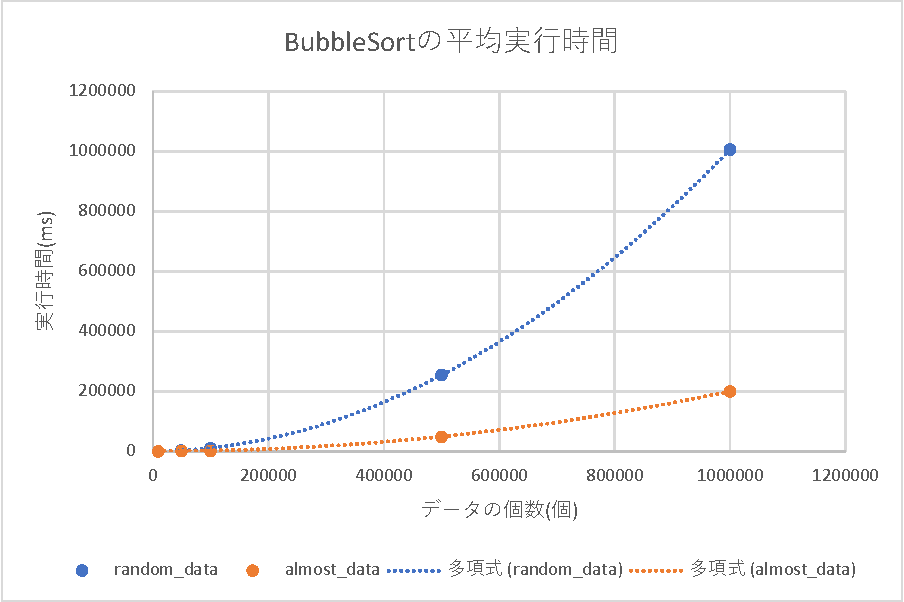
\includegraphics[keepaspectratio,width=\linewidth]{figure1.pdf}
    \caption{BubbleSortの平均実行時間}
    \label{fig:BS}
\end{figure}
\clearpage
 \begin{figure}[htbp]
    \centering
    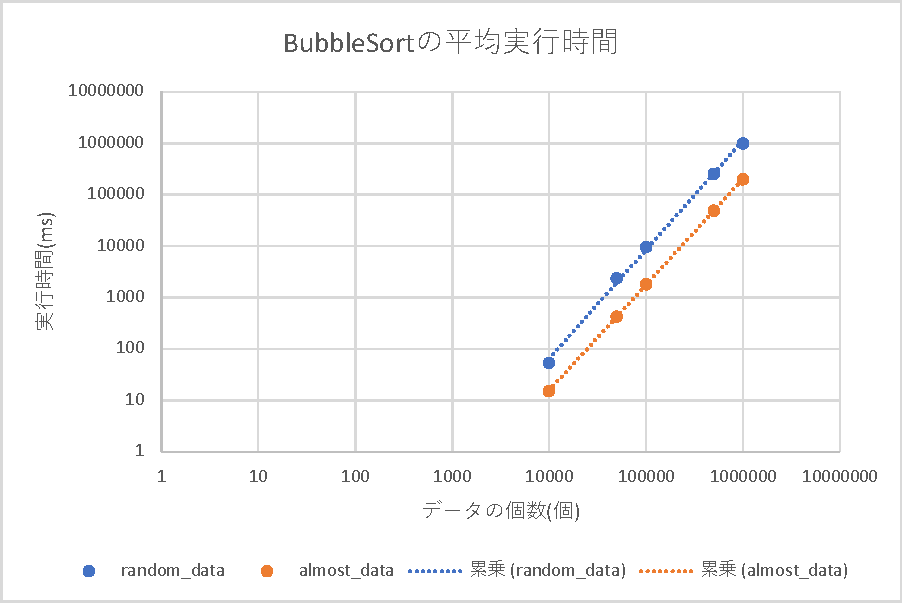
\includegraphics[keepaspectratio,width=\linewidth]{figure1loglog.pdf}
    \caption{BubbleSortの平均実行時間(両対数)}
    \label{fig:BSlog}
\end{figure}

図\ref{fig:BSlog}によると直線関係が見られ、データの個数が$10$倍になると実行時間は$10^2$倍になる。よって二乗に比例していると言える。これはバブルソートが$O(n^2)$に比例することと一致し、データがrandomな場合、almostな場合どちらでも$O(n^2)$であることが分かった。\par
また、データがほとんど整列済みであればかかる時間も大幅に削減できることが分かる。\par
しかしながら、データ数が増えると$O(n^2)$はとても効率の悪いアルゴリズムである。\par
また、当初データの格納する配列をdouble型で置いていたが、int型にキャストすることで最大1.5倍高速に動作した。これは、double型にすることでbit演算をする回数が増えたためと考えられる。

\subsection{クイックソート}
クイックソートは比較的高速に動作するアルゴリズムである。最悪実行時間$O(nlogn)$で動作し、バブルソートに比べて非常に高速に動作する。\par
以下にクイックソートの平均実行時間のグラフについて示す。
 \begin{figure}[H]
    \centering
    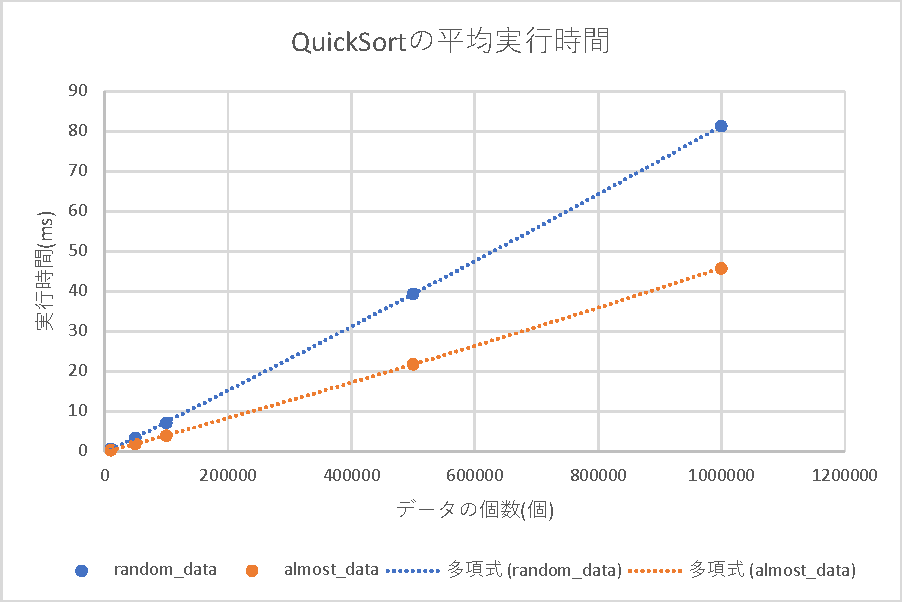
\includegraphics[keepaspectratio,width=\linewidth]{figure2.pdf}
    \caption{QuickSortの平均実行時間}
    \label{fig:QS}
\end{figure}
%\clearpage

図\ref{fig:QS}によると、ソートにかかる時間がほとんど定数倍に比例していることがわかる。実際は多項式近次と定数近似の間で$O(nlogn)$となるが、データ数が増えても1,000,000個程度ならほぼデータの数に比例して増えていると見れる。
\newpage
\subsection{基数ソート}
基数ソートは桁数を予め知っていれば、辞書的な並び替えで$O(kn)$でソートすることができ、基本的にはクイックソートの方が早い。以下に、リストによる基数ソートと、それを参考にして作成した配列による基数ソートの実行時間のグラフを示す。

 \begin{figure}[htbp]
    \centering
    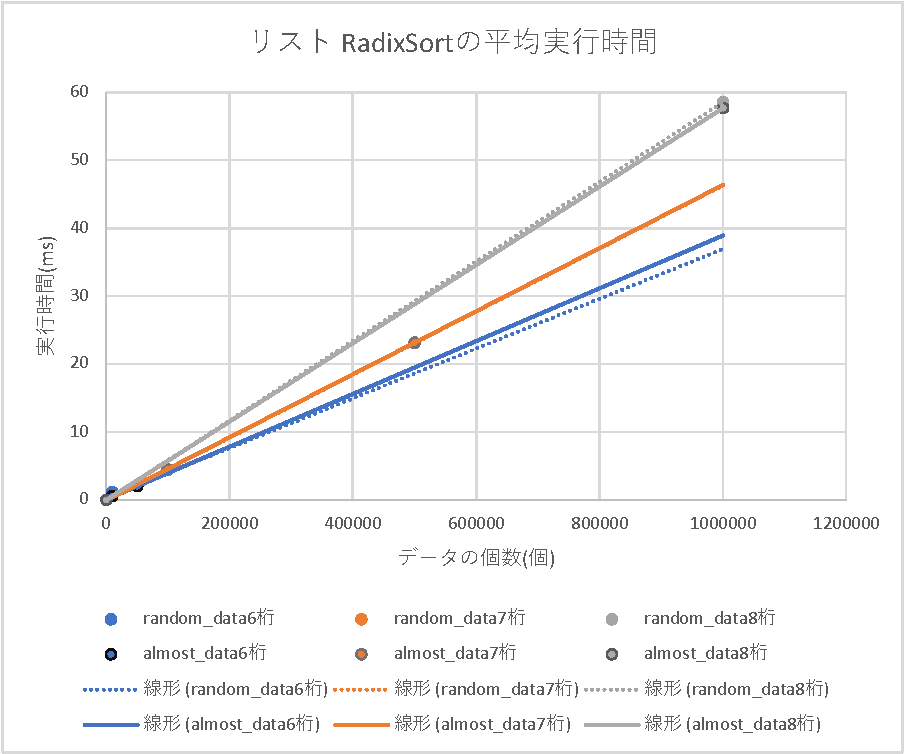
\includegraphics[keepaspectratio,width=\linewidth]{figure3.pdf}
    \caption{リスト RadixSortの平均実行時間}
    \label{fig:RS1}
\end{figure}

 \begin{figure}[H]
    \centering
    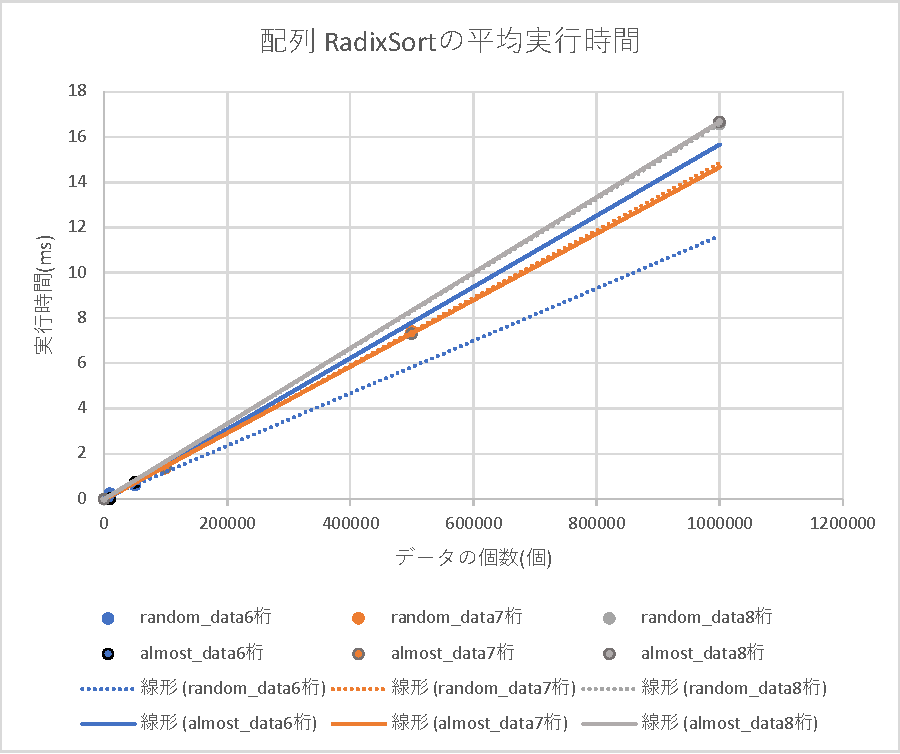
\includegraphics[keepaspectratio,width=\linewidth]{figure4.pdf}
    \caption{配列 RadixSortの平均実行時間}
    \label{fig:RS2}
\end{figure}
%\clearpage

まず、基数ソートのプログラムでは桁数を事前に把握するためグラフは桁数ごとに色分けした。\par
図\ref{fig:RS1}, 図\ref{fig:RS2}の両方で線形近似したグラフの傾きが、桁数ごとにほぼ6:7:8の比になっている。よって、$O(kn)$であることが確かめられた。\par
一部、配列のrandomデータ6桁で傾向予測にあっていない直線が見られるが、これは実行時間が極めて短いことと、データの個数の間隔が他と比べて狭いことで、少しの揺らぎが大きなずれに繋がったことが要因と考えられる。\par
次に、リストと配列を比べると、配列の方がソートで3倍程早いことが分かる。これは、データのアクセスにかかる時間が違うからと考えられる。しかし、リスト構造は使用するメモリ量が少ないので、比較的高速かつメモリの使用量を抑えるならリストの方が良いと考えられる。逆に、メモリが潤沢にある環境では配列を使って実現する方が良いと考えられる。\par
また、基数ソートはその性質上クイックソートと違い、ほとんど整列されていても関係なく常に一定のパフォーマンスで動作する。

\chapter{追加実験}
\section{実験と考察}
考察で上がった疑問を解消するために、ここではいくつかの実験を行う。
\subsection{初期の実行時間が遅い問題}
for文で配列型の基数ソートを使って1000000\_0を連続で50回ソートするプログラムを作成し実行したものと、50回ソートを単体で実行させた二つの場合を比較する。以下にその結果のグラフを示す。\par
結果のグラフを確認すると、単発の時は毎回時間がかかっているのに対し、連続して実行すると3回目から高速に動作することが分かる。
 \begin{figure}[htbp]
    \centering
    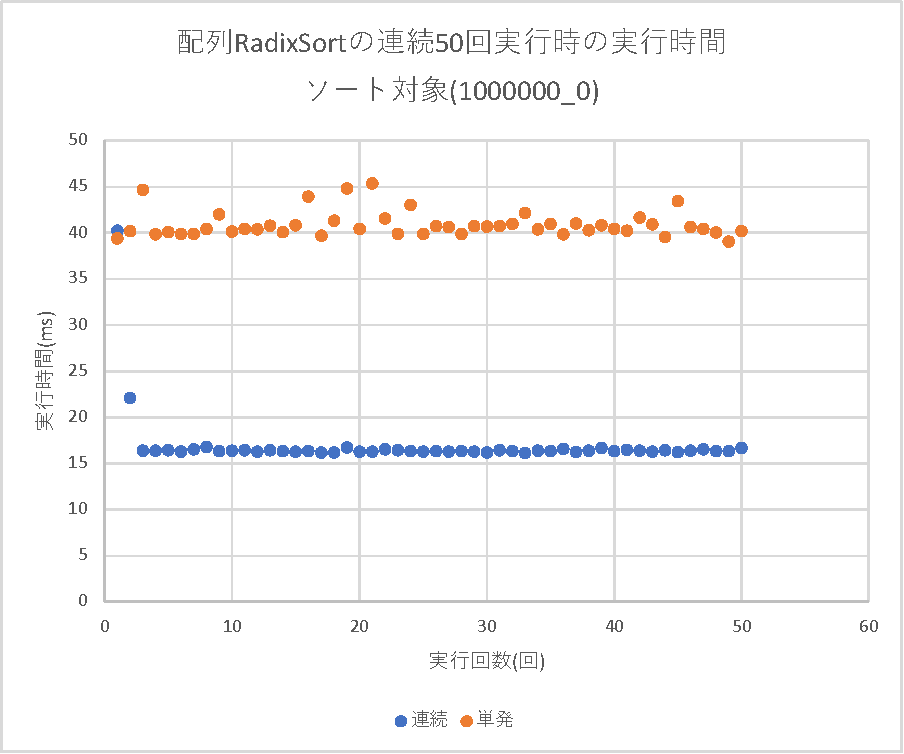
\includegraphics[keepaspectratio,width=\linewidth]{figure5.pdf}
    \caption{単発と連続したプロセスでの実行時間の比較}
    \label{fig:RS1}
\end{figure}
\clearpage
これが起きる理由としてすでに考察でもあげたが、javaのプログラムにCPUのリソースを割り当てることに時間がかかっているためだと考えられる。その裏付けとして、プログラム実行中のCPU使用率の変化についてアクティビティーモニターで確認する。すると当然だがCPU使用率は時間とともに増加し、立ち上がり初期には負荷がそこまで高くないと言うことが分かった。つまり、100\%の能力を出し切るのに時間がかかるのではないかと考えた。
参考文献 \cite{cord2} \cite{cord3} \par
また、今回の事例にはあまり当てはまらないが、インターネットライブラリから初回のロードをする際に時間がかかると言う記事があり、ローカルでも多少なりとも同じような初回ロードに時間を取られている可能性もあるのではないかと考えた。参考文献 \cite{cord4}


\subsection{ソート済みデータに対しての動作}
クイックソートはソート済みのデータに対し最良実行時間$O(n)$であるので、基数ソートの$O(kn)$より高速に動作すると予測できる。よって、最大8桁の数値データを1,000,000個用意しそれを昇順に並べたデータを用意し、クイックソート、基数ソートのどちらが早いかを計測した。上記の考察をもとにfor文で50回連続で実行した。その結果のグラフを以下に示す。
 \begin{figure}[htbp]
    \centering
    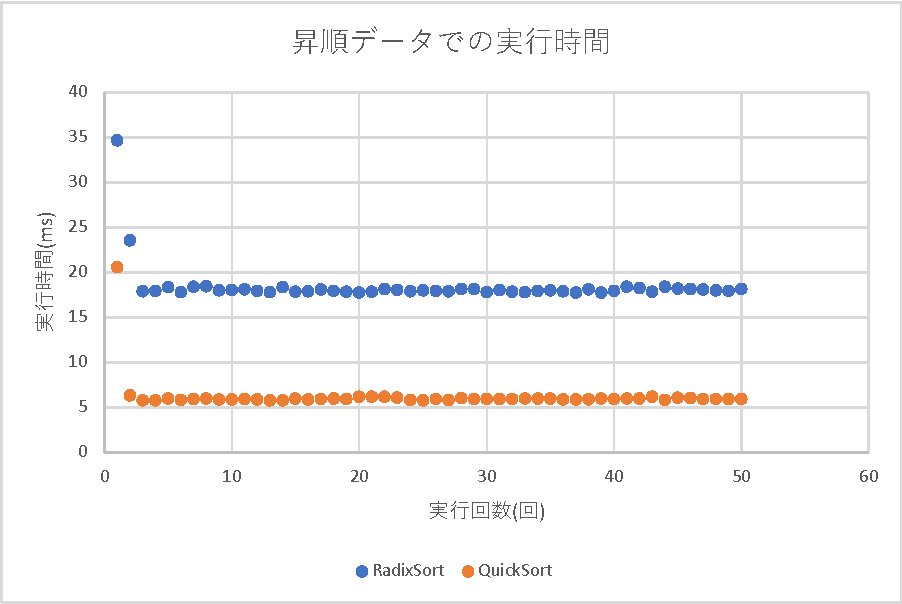
\includegraphics[keepaspectratio,width=\linewidth]{figure6.pdf}
    \caption{単発と連続したプロセスでの実行時間の比較}
    \label{fig:RS1}
\end{figure}

結果によると、やはりクイックソートの方が高速であることがわかる。つまりある程度整列されていて、適切なピボットが選択されていればクイックソートの方が早くなる可能性があると言うことが分かった。具体的にどれほどまでソートされていなかったら基数ソートより遅くなるのかは今回の実験ではわからなかったが、安定の基数ソートに比べ、伸び代が残るクイックソートも条件次第では使えると考えた。

\chapter{まとめ}
\section{今回のまとめ}
今回の実験で、数値データのソートなら配列を使った基数ソートが最も安定して早いと分かった。\\バブルソートなどは、その場ソートができ、簡単にコード書ける点では優秀だが、実際は実行時間が実用的でなく使いづらい。\\クイックソートは基数ソートに比べると遅いが、データの並び方や、ピボットの取り方によっては基数ソートより早くなるので状況に合わせて使うと良い。\par
また、データ型はdouble型よりint型の方が高速に比較でき、複数回実行するときは単発で実行するよりも連続で実行した方が高速に動作する。
\section{感想}
今回の実験ではBubbleSortの実行に最も時間がかかり、これを3回データを全て取ったのでほぼ3日分はプログラムを走らせていた。これをCSEで実行するとなると恐ろしくて止まない。しかしながらこの長い作業の中で、新たな発見や疑問が生まれ自分自身に良い経験になった。

\begin{thebibliography}{99}

\bibitem{cord1} 基数ソート(Radix Sort)\url{https://qiita.com/yp2211/items/683fa423b3f40a871064} 2023/6/18
\bibitem{cord2} 第3回 プロセスとスレッド:Windows OS入門
 \url{https://atmarkit.itmedia.co.jp/ait/spv/1410/30/news150.html} 2023/6/20
\bibitem{cord3} Linuxのしくみを学ぶ - プロセス管理とスケジューリング \url{https://syuu1228.github.io/process_management_and_process_schedule/process_management_and_process_schedule.html} 2023/6/20
\bibitem{cord4} AWS LambdaのJavaは遅い? \url{https://qiita.com/moritalous/items/632333088948aad7f8c9} 2023/6/20


\end{thebibliography}



\end{document}  